\documentclass[border=10pt]{standalone}

\usepackage{tikz}
\usepackage{amsmath}

\usetikzlibrary{
    positioning,
    arrows.meta,
    fit,
    backgrounds,
    shapes.geometric,
    calc
}

\pagestyle{empty}

% ============================================================================
% PART I: FRONTENDS -> CROSS-MODAL ATTENTION
% ============================================================================
\begin{document}
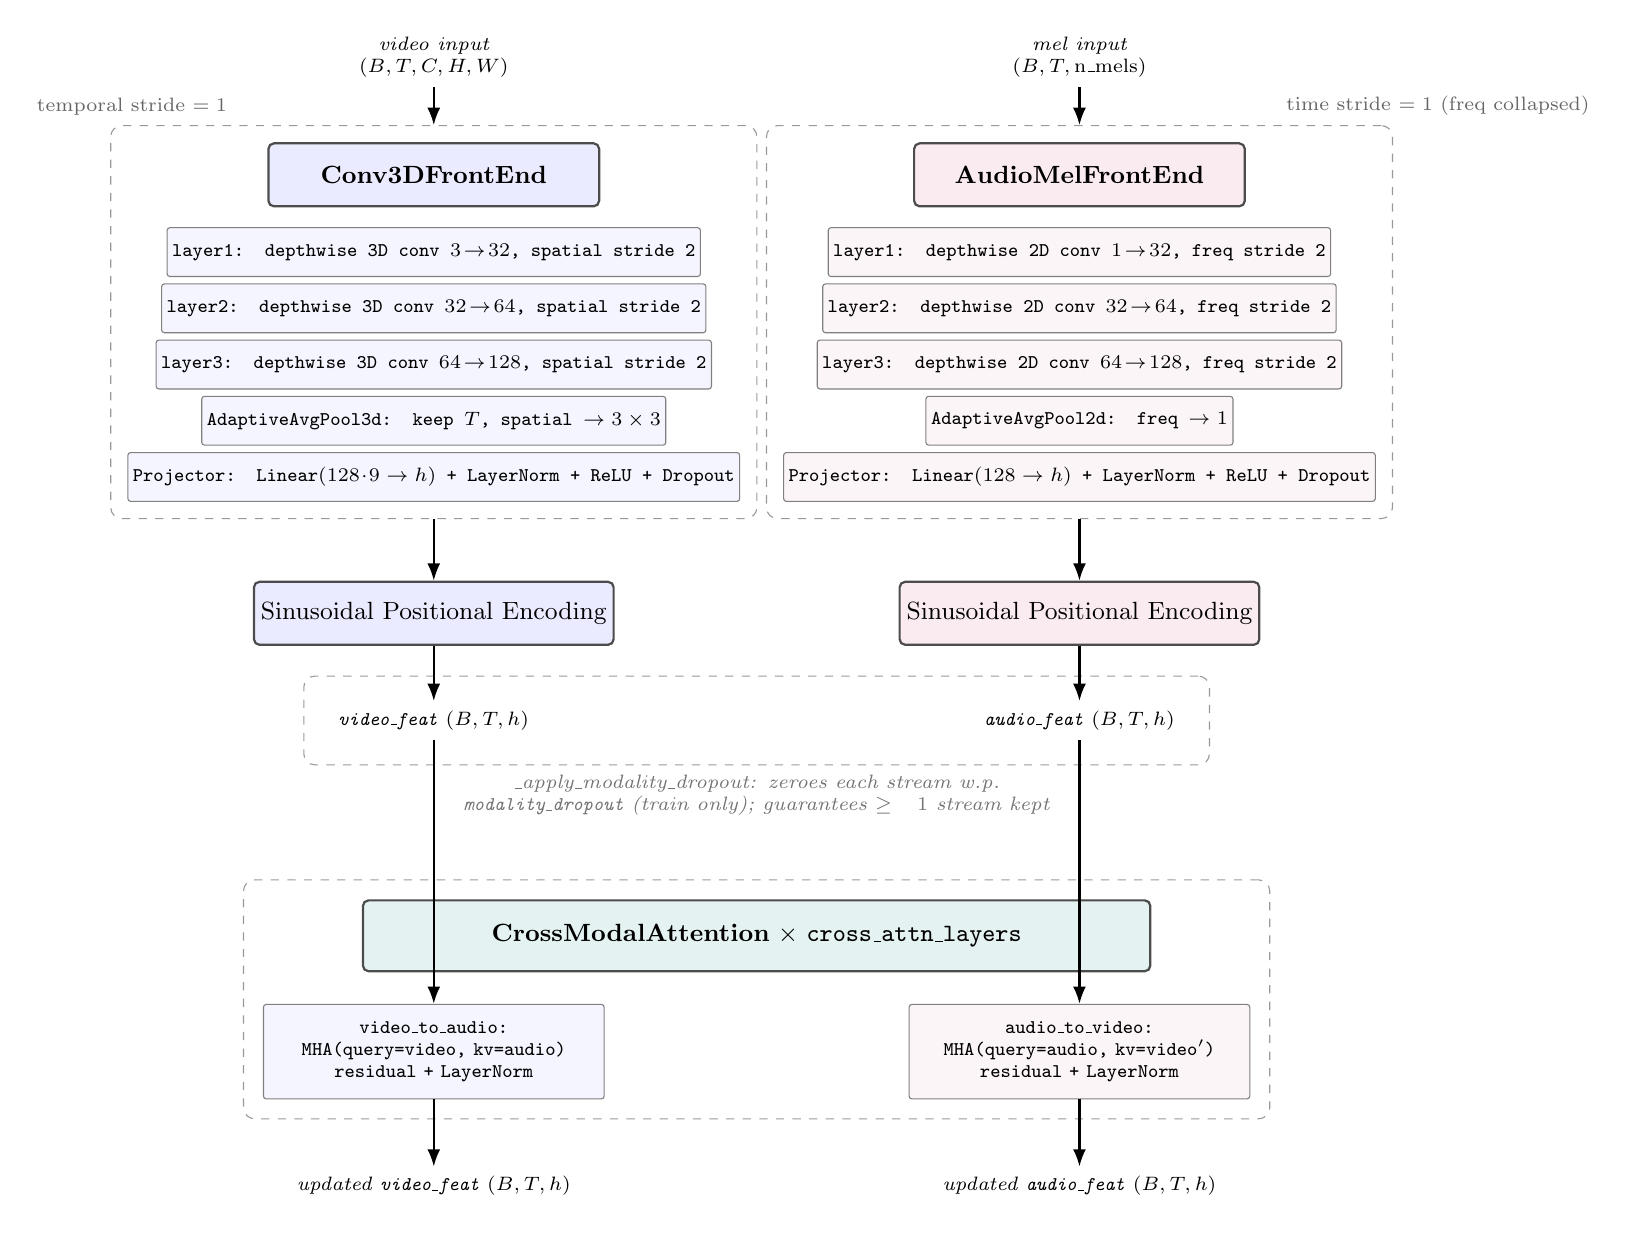
\begin{tikzpicture}[
    font=\small,
    node distance=5mm and 18mm,
    block/.style={
        rectangle, draw=black!70, thick, rounded corners=2pt,
        fill=blue!8, minimum width=42mm, minimum height=8mm,
        align=center, inner sep=2.5pt
    },
    ablock/.style={
        rectangle, draw=black!70, thick, rounded corners=2pt,
        fill=purple!8, minimum width=42mm, minimum height=8mm,
        align=center, inner sep=2.5pt
    },
    subblock/.style={
        rectangle, draw=black!50, rounded corners=1pt,
        fill=blue!4, minimum width=39mm, minimum height=6.2mm,
        align=center, font=\scriptsize\ttfamily, inner sep=1.8pt
    },
    asubblock/.style={
        rectangle, draw=black!50, rounded corners=1pt,
        fill=purple!4, minimum width=39mm, minimum height=6.2mm,
        align=center, font=\scriptsize\ttfamily, inner sep=1.8pt
    },
    centerblock/.style={
        rectangle, draw=black!70, thick, rounded corners=2pt,
        fill=teal!10, minimum width=100mm, minimum height=9mm,
        align=center, inner sep=2.5pt
    },
    iolabel/.style={
        rectangle, draw=none, fill=none, align=center, font=\scriptsize\itshape
    },
    groupbox/.style={
        rectangle, draw=black!40, dashed, rounded corners=4pt, inner sep=6pt
    },
    arr/.style={-{Latex[length=2.2mm]}, thick},
    thinarr/.style={-{Latex[length=1.8mm]}, thin},
    every label/.style={font=\scriptsize}
]

% Inputs
\node[iolabel] (video_in) at (-41mm,0) {video input\\ $(B,T,C,H,W)$};
\node[iolabel] (mel_in) at (41mm,0)
    {mel input\\ $(B,T,\mathrm{n\_mels})$};

% Video frontend
\node[block, below=7mm of video_in] (v_front_title) {\textbf{Conv3DFrontEnd}};
\node[subblock, below=2.5mm of v_front_title] (v_l1)
    {layer1: depthwise 3D conv $3\!\to\!32$, spatial stride 2};
\node[subblock, below=0.8mm of v_l1] (v_l2)
    {layer2: depthwise 3D conv $32\!\to\!64$, spatial stride 2};
\node[subblock, below=0.8mm of v_l2] (v_l3)
    {layer3: depthwise 3D conv $64\!\to\!128$, spatial stride 2};
\node[subblock, below=0.8mm of v_l3] (v_pool)
    {AdaptiveAvgPool3d: keep $T$, spatial $\to3\times3$};
\node[subblock, below=0.8mm of v_pool] (v_proj)
    {Projector: Linear$(128\!\cdot\!9\to h)$ + LayerNorm + ReLU + Dropout};
\node[groupbox, fit=(v_front_title)(v_l1)(v_l2)(v_l3)(v_pool)(v_proj),
      label={[font=\scriptsize,text=black!60]above left:temporal stride $=1$}] (v_frontbox) {};

% Audio frontend
\node[ablock, below=7mm of mel_in] (a_front_title) {\textbf{AudioMelFrontEnd}};
\node[asubblock, below=2.5mm of a_front_title] (a_l1)
    {layer1: depthwise 2D conv $1\!\to\!32$, freq stride 2};
\node[asubblock, below=0.8mm of a_l1] (a_l2)
    {layer2: depthwise 2D conv $32\!\to\!64$, freq stride 2};
\node[asubblock, below=0.8mm of a_l2] (a_l3)
    {layer3: depthwise 2D conv $64\!\to\!128$, freq stride 2};
\node[asubblock, below=0.8mm of a_l3] (a_pool)
    {AdaptiveAvgPool2d: freq $\to1$};
\node[asubblock, below=0.8mm of a_pool] (a_proj)
    {Projector: Linear$(128\to h)$ + LayerNorm + ReLU + Dropout};
\node[groupbox, fit=(a_front_title)(a_l1)(a_l2)(a_l3)(a_pool)(a_proj),
      label={[font=\scriptsize,text=black!60]above right:time stride $=1$ (freq collapsed)}] (a_frontbox) {};

% Positional encodings and feature labels -- deliberately more vertical space
\node[block, below=10mm of v_proj] (v_posenc) {Sinusoidal Positional Encoding};
\node[ablock, below=10mm of a_proj] (a_posenc) {Sinusoidal Positional Encoding};
\node[iolabel, below=7mm of v_posenc] (v_feat) {\texttt{video\_feat} $(B,T,h)$};
\node[iolabel, below=7mm of a_posenc] (a_feat) {\texttt{audio\_feat} $(B,T,h)$};

% Modality dropout annotation
\node[groupbox, fit=(v_feat)(a_feat), inner sep=9pt,
      label={[font=\scriptsize\itshape, text=black!55, text width=110mm, align=center]below:\_apply\_modality\_dropout: zeroes each stream w.p. \texttt{modality\_dropout} (train only); guarantees $\ge1$ stream kept}] (moddrop) {};

% Cross-modal attention -- widely separated and equal-height blocks
\node[centerblock, below=17mm of moddrop] (cross_title)
    {\textbf{CrossModalAttention} $\times$ \texttt{cross\_attn\_layers}};
\node[subblock, below=4mm of cross_title, xshift=-41mm,
      text width=42mm, minimum width=42mm, minimum height=12mm] (v2a)
    {video\_to\_audio: MHA(query=video, kv=audio)\\ residual + LayerNorm};
\node[asubblock, below=4mm of cross_title, xshift=41mm,
      text width=42mm, minimum width=42mm, minimum height=12mm] (a2v)
    {audio\_to\_video: MHA(query=audio, kv=video$'$)\\ residual + LayerNorm};
\node[groupbox, fit=(cross_title)(v2a)(a2v), inner sep=7pt] (crossbox) {};

% Outputs aligned on the same horizontal level
\node[iolabel] (v_feat2) at ([yshift=-11mm]v2a.south)
    {updated \texttt{video\_feat} $(B,T,h)$};
\node[iolabel] (a_feat2) at ([yshift=-11mm]a2v.south)
    {updated \texttt{audio\_feat} $(B,T,h)$};

% Arrows
\draw[arr] (video_in) -- (v_frontbox.north);
\draw[arr] (mel_in) -- (a_frontbox.north);
\draw[arr] (v_frontbox.south) -- (v_posenc.north);
\draw[arr] (a_frontbox.south) -- (a_posenc.north);
\draw[arr] (v_posenc.south) -- (v_feat.north);
\draw[arr] (a_posenc.south) -- (a_feat.north);

% Straight, uncrowded inputs into the two cross-attention blocks
\draw[arr] (v_feat.south) -- (v2a.north);
\draw[arr] (a_feat.south) -- (a2v.north);

\draw[arr] (v2a.south) -- (v_feat2.north);
\draw[arr] (a2v.south) -- (a_feat2.north);

\end{tikzpicture}
\end{document}
